\documentclass{article}
\usepackage[a4paper]{geometry}
\usepackage{graphicx}
\usepackage{listings}
\usepackage[utf8]{inputenc}
\author{Alessandro Rosso, Elia Migliore, Franco Ruggeri}
\title{Relazione Seconda Esercitazione Sistemi Elettronici}
\date{15 December 2017}

\begin{document}

\section{Introduzione}
In questa esercitazione sperimentale di sistemi elettronici abbiamo misurato il comportamento di due amplificatori reali, uno non invertente e uno invertente.\\Abbiamo quindi poi confrontare i risultati ottenuti dalle misure con quelli ottenuti dai calcoli teorici, osservando i limiti che le semplificazioni teoriche inducono.

\section{Strumenti}
Per effettuare questa esercitazione abbiamo dovuto utilizzare quindi:
\begin{itemize}
	\item \textbf{Generatore da banco}
	\item \textbf{Generatore di segnali}
    \item \textbf{Oscilloscopio digitale}
	\item \textbf{Scheda con amplificatori "A2"}
\end{itemize}

\subsection{Generatore banco}

Il generatore da banco è stato configurato in modo che erogasse 12V sia sull'uscita 1 che sull'uscita 2.
\\
Si è quindi collegato un cavo con entrambi i connettori a banana in modo che cortocircuitasse il GND della prima uscita e il +12V della seconda uscita, così da poterlo utilizzare come \textbf{generatore duale}.\\ Su questo cavo banana-banana si è poi anche inserito il connettore a banana verde ( potenziale a 0V ) che usciva dal connettore collegato alla porta J8 presente sulla scheda con gli amplificatori.\\
I connettori a banana rosso e nero che uscivano dal connettore connesso a J8 sono poi stati collegati alle uscite 1 - +12V e 2 - GND del generatore da banco, rispettivamente.\\
Abbiamo così ottenuto una differenza di potenziale pari a +24V tra i cavi rosso e nero del connettore di alimentazione della scheda "A2", +12V tra il rosso e il verde e -12V tra il verde e il nero.

\subsection{Generatore di segnali}
Il generatore di segnali è stato collegato attraverso un connettore coassiale sia all'uscita 50ohm (del generatore di segnali) sia all'ingresso J1 della scheda "A2".

\subsection{Oscilloscopio digitale}
\subsubsection{Canale 1} Il canale 1 dell'oscilloscopio è stato collegato attraverso un connettore da coassiale (ingresso verso oscillosopio) a morsetti rosso e nero, collegati a J4 e J5 (della scheda "A2") rispettivamente.
\subsubsection{Canale 2} Il canale 2 dell'oscilloscopio è stato collegato sempre attraverso un connettore da coassiale (ingresso verso oscillosopio) a morsetti rosso e nero, collegati a J6 e J7 rispettivamente.

\section{Amplificatore non invertente senza elementi reattivi}
Per la prima parte dell'esercitazione siamo andati ad analizzare l'amplificatore non invertente presente sulla scheda.

\subsection{Calcoli teorici}
Per questa prima parte dell'esercitazione non era richiesto il calcolo dei valori teorici in quanto già forniti nei dati dell'esercitazione.
Sono quindi quà riportati:
\begin{itemize}
\item \large $R_{in} = (10.00 \pm 0.50)k\Omega$
\item \large $R_{out} = (1.00 \pm 0.05)k\Omega$
\item \large ${|A_{v}|}_{dB} = (20.0 \pm ...)$
\end{itemize}
\subsection{Predisposizione scheda}
Per poter utilizzare l'amplificatore non invertente bisognava predisporre la scheda andando a commutare degli \textbf{interruttori} presenti su di essa, nello specifico abbiamo settato gli interruttori nel seguente modo:
\begin{itemize}
	\item \textbf{S1}: Posizione 2 \textit{Mettendo S1 in \textbf{posizione 2} si collega l'ingresso (l'uscita del generatore di segnale) all'ingresso dell'\textbf{amplificatore non invertente}.\\Viceversa se posto in \textbf{posizione 1} si collegherebbe J1 all'ingresso dell'\textbf{amplificatore invertente}.}
	\item \textbf{S2}: Posizione 2 \textit{Mettendo S2 in \textbf{posizione 2} si collega l'uscita dell'\textbf{amplificatore non invertente} al "circuito di uscita", viceversa se si mette S2 in \textbf{posizione 1} si collega l'uscita dell'\textbf{amplificatore invrtente} al circuito di uscita}
	\item \textbf{S3}: Posizione 2 \textit{Commutando S3 in \textbf{posizione 1} insieme a S4 in posizione 1 si va ad inserire il condensatore \textbf{C10} in "serie alla resistenza di ingresso" (e in parallelo a C5) dell'amplificatore}
	\item \textbf{S4}: Posizione 2 \textit{Commutando S4 in \textbf{posizione 1} si andrebbe a inserire \textbf{C5} in "serie alla resistenza di ingresso" (e in parallelo a C10 se S3 = 1)}
	\item \textbf{S5}: Posizione 2
	\textit{Mettendo S5 in \textbf{posizione 1} si va ad inserire la resistenza \textbf{R9} in serie al circuito di ingresso}
	\item \textbf{S6}: Posizione 1
	 \textit{Mettendo S6 in \textbf{posizione 2} sia ndrebbe ad inserire \textbf{R10} in serie al circuito di uscita}
	\item \textbf{S7}: Posizione 1
	 \textit{Mettendo S7 in \textbf{posizione 2} sia ndrebbe ad inserire \textbf{R11} in serie al circuito di uscita}
	\item \textbf{S8}: Posizione 1
	 \textit{Mettendo S8 in \textbf{posizione 2} sia ndrebbe ad inserire \textbf{C6} in serie al circuito di uscita}
	\item \textbf{S9}: Posizione 1
	 \textit{Mettendo S9 in \textbf{posizione 2} sia ndrebbe ad inserire \textbf{C9} in serie al circuito di uscita}
\end{itemize}

\subsection{Misura guadagno}
\subsubsection{Impostazione segnale generatore segnale}
Per effettuare la misura di guadagno è richiesto di impostare il generatore di segnale in modo che generi un \textbf{segnale} di uscita \textbf{sinusoidale} di \textbf{frequenza} pari a \textbf{800Hz} e \textbf{valore di picco-picco} di \textbf{1V}.

\subsubsection{Segnale misurato}
Passiamo ora all'analisi dei valori misurati attraverso l'oscilloscopio.\\Dall'analisi dell'uscita visualizzata sul display dell'oscilloscopio possiamo calcolare una \textbf{tensione di ingresso} pari a \large $V_s = (980 \pm 39)$mV \normalsize (in quanto possiamo leggere il risultato come 4.9 divisioni con una scala di 200mV a divisione).\\
Per quanto riguarda la \textbf{tensione di uscita} invece leggiamo un valore di \large $V_u = (8.40 \pm 0.36)$V \normalsize (ottenuto da 4.2 divisione con una scala di 2.00V per divisione).
\subsubsection{Calcolo guadagno}
Ottemiamo quindi un \textbf{guadagno} pari a:\\ \large $A_v = \frac{V_s}{V_u} = (8.57 \pm 0.71)$ \normalsize \\Che, espresso \textbf{in decibel} diventa:\\ \large $ |A_v|_{dB} = (18.7 \pm 1.7)$dB \normalsize

\subsection{Misura della resistenza di ingresso}
\subsubsection{Metodo di misura per le resistenze}
Per poter effettuare le misure di resistenza si è scelto di sfruttare l'inserimento di una \textbf{resistenza in serie} al circuito di ingresso, R9 ("inseribile" tramite l'interruttore S5 ???).\\Calcolando quindi la tensione di uscita senza resistenza R9 in serie si ottiene:\\
\large $V_{u} = A_{v} * V_{in}$ \normalsize \\ Invece se si inserisce R9 in serie commutando la posizione di S5???? si ottiene:\\
\large $ V_{u}^{'} = A_{v} * V_{in} * \frac{R_{in}}{R_{in} + R_9} $ \normalsize \\ Facendo il rapporto \large $\frac{V_{u}^{'}}{{V_u}}$ \normalsize si ottiene quindi: \\ \large $R_{in} = \frac{R_9 * V_{u}^{'}}{V_u - V_{u}^{'}} $

\subsubsection{Calcolo resistenza ingresso}
I valori numerici misurati sono i seguenti:
\begin{itemize}
	\item \large $R_{9} = 10k\Omega \pm 1\%$
	\item \large $V_{u} = (8.40 \pm 0.36)V$
	\item \large $V_{u}^{'} = (4.40 \pm 0.18)V$
\end{itemize}
Inserendoli nella formula precedente otteniamo quindi un valore di: \\ \large $R_{in} = (11.0 \pm 2.0)k\Omega$

\subsection{Misura della resistenza di uscita}
\subsubsection{Metodo di misura per le resistenze}
\normalsize Per poter effettuare le misure di resistenza si è scelto di sfruttare l'inserimento di una \textbf{resistenza in serie} al circuito di uscita, R10 ("inseribile" tramite l'interruttore S6 ???).\\Calcolando quindi la tensione di uscita senza resistenza R10 in serie si ottiene:\\
\large $V_{u} = A_{v} * V_{in}$ \normalsize \\ Invece se si inserisce R10 in serie commutando la posizione di S6???? si ottiene:\\
\large $ V_{u}^{'} = A_{v} * V_{in} * \frac{R_{10}}{R_{10} + R_u} $ \normalsize \\ Facendo il rapporto \large $\frac{V_{u}^{'}}{{V_u}}$ \normalsize si ottiene quindi: \\ \large $R_{in} = R_{10} * (\frac{V_{u}-V_{u}^{'}}{V_{u}^{'}}) $ \normalsize
\subsubsection{Calcolo resistenza uscita}
I valori numerici misurati sono i seguenti:
\begin{itemize}
	\item \large $R_{10} = 1k\Omega \pm 5\%$
	\item \large $V_{u} = (8.40 \pm 0.36)V$
	\item \large $V_{u}^{'} = (4.20 \pm 0.18)V$
\end{itemize}
Inserendoli nella formula precedente otteniamo quindi un valore di: \\ \large $R_{u} = (1.0 \pm 0.23)k\Omega$

\subsection{Confronto valori teorici e valori ottenuti dalle misure}
I valori misurati sono tutti compatibili con i valori teorici.

\section{Amplificatore non invertente con elementi reattivi}
\subsection{Calcoli teorici}
La funzione presenta un polo nell'origine, e due poli a circa $1.2kHz$ e $16kHz$.
Per il calcolo dei valori teorici abbiamo sfruttato un semplice script in python il cui codice è qui riportato:
\begin{lstlisting}[language=Python, breaklines=true]
import math
import matplotlib.pyplot as plt

debug = False

#define gain value of the amplfier
a = 9.33
#define the absolute error of gain 10%
da = 0.933
#define the value of the resistor in series of the output port of the amplifier
ru = 1000
#define the absolute error of Ru 5%
dru = 0.05*ru
#define the value of C6
csei = 10E-9
#define the absolute error of C6 20%
dcsei = 0.2*csei
#define value of Cin (sum of the capacitors in input)
cin = 13.3 * 1E-9
#define the error of Cin
dcin = 0.2*cin
#define Rin
rin = 10E3
#define the error of Rin 5%
drin = 0.05*rin
#define the error of the frequency
df = 0
#define k, a usefull costant
k = 20/math.log(10)
#calc the frequency of the first pole
fp = 1/(2 * math.pi * ru * csei)
#calc the frequency of the second pole
fp2 = 1/(2 * math.pi * rin * cin)
#calc the error of the first pole
dfp = 2*math.pi*math.pow(fp,2)*((ru * dcsei)+(dru * csei))
if debug: print ("fp %f") % fp
if debug: print ("dfp %f") % dfp
#calc the error of the second pole
dfp2 = 2*math.pi*math.pow(fp2,2)*((rin * dcin)+(cin * drin))
if debug: print ("fp2 %f") % fp2
if debug: print ("dfp2 %f") % dfp2
#calc the costant gain value in dB
avdb = 20*math.log(a * cin * rin,10)
#calc the error costant gain value in dB
davdb = k*((da/a)+(drin/rin)+(dcin/cin))
if debug: print ("av dB %f") % avdb
if debug: print ("dav dB %f") % davdb

#define the frequency where we'll calc the gain and the error
f = [300,1000,3000,10000,30000,100000,300000,1000000]

x=[]
dx=[]
ph=[]
dph=[]

#Valori ottenuti dalle misure (necessarie per la generazione del diagramma di bode)
mis=[7.00,15.30,18.02,17.20,12.21,2.92,-8.89,-26.9]
dmis=[0.7,0.67,0.62,0.63,0.74,0.69,0.79,1.0]
misp=[0.00121,0.000754,0.000170,0.503,-1.13,-1.89,-3.77,-3.14]
dmisp=[0.00006,0.000046,0.000022,0.22,0.06,0.10,0.17,0.19]

#for each frequency defined above
for i in f:
	#calc the modulo of the first pole at a specific frequency
	mfp = math.sqrt(1+math.pow(i/fp,2))
	if debug: print("mfp %f") % mfp
	#calc the modulo of the second pole at a specific frequency
	mfp2 = math.sqrt(1+math.pow(i/fp2,2))
	if debug: print("mfp2 %f") % mfp2
	#calc the gain of the amplifier at a specific frequency
	av = avdb + (20*math.log(2*math.pi*i,10)) - (20*math.log(mfp,10)) - (20*math.log(mfp2,10))
	#calc a usefull costant for the first pole
	kp = (k*i)/(math.pow(fp,2)*mfp)
	if debug: print ("kp %f") % kp
	#calc a usefull costant for the second pole
	kp2 = (k*i)/(math.pow(fp2,2)*mfp2)
	if debug: print ("kp2 %f") % kp2
	#calc the absolute error of the gain given by the frequency error
	ddf = (k/i) * df
	if debug: print ("ddf %f") % ddf
	#calc the absolute error of the gain given by the first pole error
	ddfp = (kp/mfp)*(df + ((i/fp)*dfp))
	if debug: print ("ddfp %f") % ddfp
	#calc the absolute error of the gain given by the second pole error
	ddfp2 = (kp2/mfp2)*(df + ((i/fp2)*dfp2))
	if debug: print ("ddfp2 %f") % ddfp2
	#calc the absolute error of the gain (summing the error calculated before)
	dav = davdb + ddf + ddfp + ddfp2
	#calc of the phase
	pi = math.atan( (1 - (math.pow(i,2)/(fp*fp2))) / (i*(fp2 + fp)/(fp2*fp)))
        x.append(round(av,2))
        dx.append(round(dav,2))
        ph.append(round(pi,2))
        dph.append(round(0.00,2))
	print("@%dHz\tAv = (%.2f +- %.2f)dB\tPhase = (%.2f +- %.2f)rad") % (i, x[len(x)-1], dx[len(x)-1],ph[len(ph)-1],dph[-1])

#Rappresento graficamente risultati ottenuti con incertezze
plt.subplot(211)
plt.errorbar(f,x,yerr=dx,color="b",linestyle="--")
plt.errorbar(f,mis,yerr=dmis,color="r",linestyle=":")
plt.xscale('log')
plt.subplot(212)
plt.errorbar(f,ph,yerr=dph,color="b",linestyle="--")
plt.errorbar(f,misp,yerr=dmisp,color="r",linestyle=":")
plt.xscale('log')
plt.show()
\end{lstlisting}

\subsection{Misure in frequenza}
\subsubsection{Tabella delle misure}
% tabella aggiunta da elia
Tabella:
\\
\begin{table}[]
\centering
\label{my-label}
\renewcommand{\arraystretch}{1.5}
\begin{tabular}{|c|c|c|c|}
\hline $f$ & $\Delta_\phi$ & ${|A_v|}_{calcolato}$ & ${|A_v|}_{misurato}$
\\
\hline $300Hz$ & $(1.21 \pm 0.06)*10^{-3} rad$ & $(7.1 \pm 3.2) $ & $ (7.00 \pm 0.70) $\\
\hline $1kHz$ & $(7.54 \pm 0.46)*10^{-4} rad$ & $(15.52 \pm 3.9)$ & $ (15.30 \pm 0.67) $\\
\hline $3kHz$ & $(1.70 \pm 0.22)*10^{-4} rad$ & $(18.6 \pm 5.0)$ & $ (18.02 \pm 0.62) $\\
\hline $10kHz$ & $(5.03 \pm 0.22)*10^{-1} rad$ & $(17.9 \pm 5.8)$ & $ (17.20 \pm 0.63) $\\
\hline $30kHz$ & $(1.13 \pm 0.06) rad$ & $(12.8 \pm 6.9)$ & $ (12.21 \pm 0.74) $\\
\hline $100kHz$ & $(1.89 \pm 0.10) rad$ & $(3.32 \pm 7.3)$ & $ (2.92 \pm 0.69) $\\
\hline $300kHz$ & $(3.77 \pm 0.17) rad$ & $(-6.12 \pm 7.38)$ & $ (-8.87 \pm 0.79) $\\
\hline $1MHz$ & $(3.14 \pm 0.19) rad$ & $(-16.57 \pm 7.38)$ & $ (-26.9 \pm 1.0) $\\
\hline
\end{tabular}
\\
\end{table}
\begin{figure}
  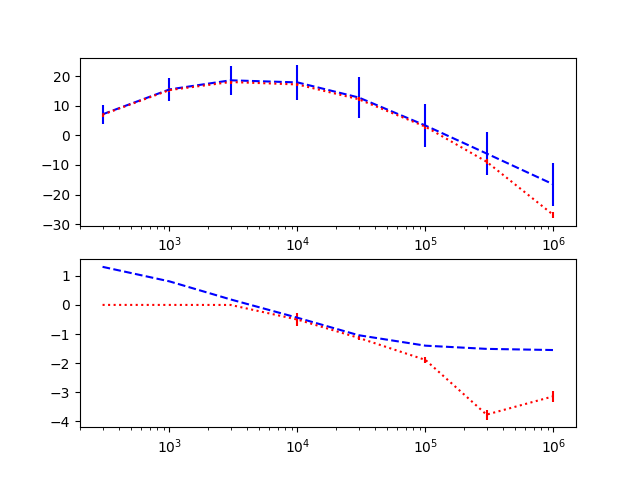
\includegraphics[width=\textwidth]{Bode.png}
  \caption{In rosso i valori misurati; In blu quelli teorici; Sopra il modulo, sotto la fase}
  \label{fig:bode1}
\end{figure}

\subsubsection{Note}
Abbiamo riscontrato un elevato livello di rumore con le misure prese ad una frequenza di 1MHz (vedere imagine sotto), già a 300KHz si riscontravano alcuni disturbi.

\subsection{Confronto valori teorici e valori ottenuti dalle misure}
I valori misurati non si discostano molto dai valori teorici calcolati. Soprattutto si può vedere che tutte le misure risultino compatibili con quelle teoriche. Solo quella alla frequenza di 1MHz risulta non compatibile, molto probabilmente a causa dell'elevato disturbo riscontrato in fase di misura del segnale di ingresso e segnale di uscita.

\section{Amplificatore invertente}
\normalsize
\subsection{Misura guadagno}
\subsubsection{Impostazione segnale generatore segnale}
Per effettuare la misura di guadagno è richiesto di impostare il generatore di segnale in modo che generi un \textbf{segnale} di uscita \textbf{sinusoidale} di \textbf{frequenza} pari a \textbf{1KHz} e \textbf{valore di picco-picco} di \textbf{1V}.

\subsubsection{Segnale misurato}
Passiamo ora all'analisi dei valori misurati attraverso l'oscilloscopio.\\Dall'analisi dell'uscita visualizzata sul display dell'oscilloscopio possiamo calcolare una \textbf{tensione di ingresso} pari a \large $V_s = (980 \pm 39)$mV \normalsize (in quanto possiamo leggere il risultato come 4.9 divisioni con una scala di 200mV a divisione).\\
Per quanto riguarda la \textbf{tensione di uscita} invece leggiamo un valore di \large $V_u = (10.0 \pm 0.39)$V \normalsize (ottenuto da 5 divisione con una scala di 2.00V per divisione).
\subsubsection{Calcolo guadagno}
Ottemiamo quindi un \textbf{guadagno} pari a:\\ \large $A_v = \frac{V_s}{V_u} = (10.20 \pm 0.80)$ \normalsize \\Che, espresso \textbf{in decibel} diventa:\\ \large $ |A_v|_{dB} = (20.2 \pm 1.6)$dB \normalsize
\subsection{Misura resistenza di ingresso}
Per la misura della resistenza di ingresso procediamo come per l'amplificatore non invertente.
\subsubsection{Misure ottenute}
I valori numerici misurati sono i seguenti:
\begin{itemize}
	\item \large $R_{9} = 10k\Omega \pm 1\%$
	\item \large $V_{u} = (10.0 \pm 0.39)V$
	\item \large $V_{u}^{'} = (6.00 \pm 0.31)V$
\end{itemize}
Inserendoli nella formula precedente otteniamo quindi un valore di: \\ \large $R_{in} = (15.0 \pm 3.5)k\Omega$
\subsubsection{Note}
Confrontando il valore ottenuto con il valore nominale di $(15.00 \pm 0.75)kHz$ vediamo che le misure sono compatibili.
\subsection{Misura resistenza di uscita}
Anche per la misura della resistenza di uscita procediamo come per l'amplificatore non invertente.
\subsubsection{Misure ottenute}
I valori numerici misurati sono i seguenti:
\begin{itemize}
	\item \large $R_{10} = 1k\Omega \pm 5\%$
	\item \large $V_{u} = (10.0 \pm 0.39)V$
	\item \large $V_{u}^{'} = (10.0 \pm 0.39)V$
\end{itemize}
\subsubsection{Note}
Si denota vedendo le misure che l'inserimento della resistenza $R_{10}$ è completamente ininfluente per quanto riguarda la tensione di uscita.\\Questo implica che il valore di $R_{10}$ sia completamente 
trascurabile rispetto a $R_{u}$.
\subsection{Verifica inversione di fase}
Come si denota dall'immagine, la fase del segnale di uscita è ritardata di 180 gradi rispetto a quella del segnale di ingresso
\begin{figure}
  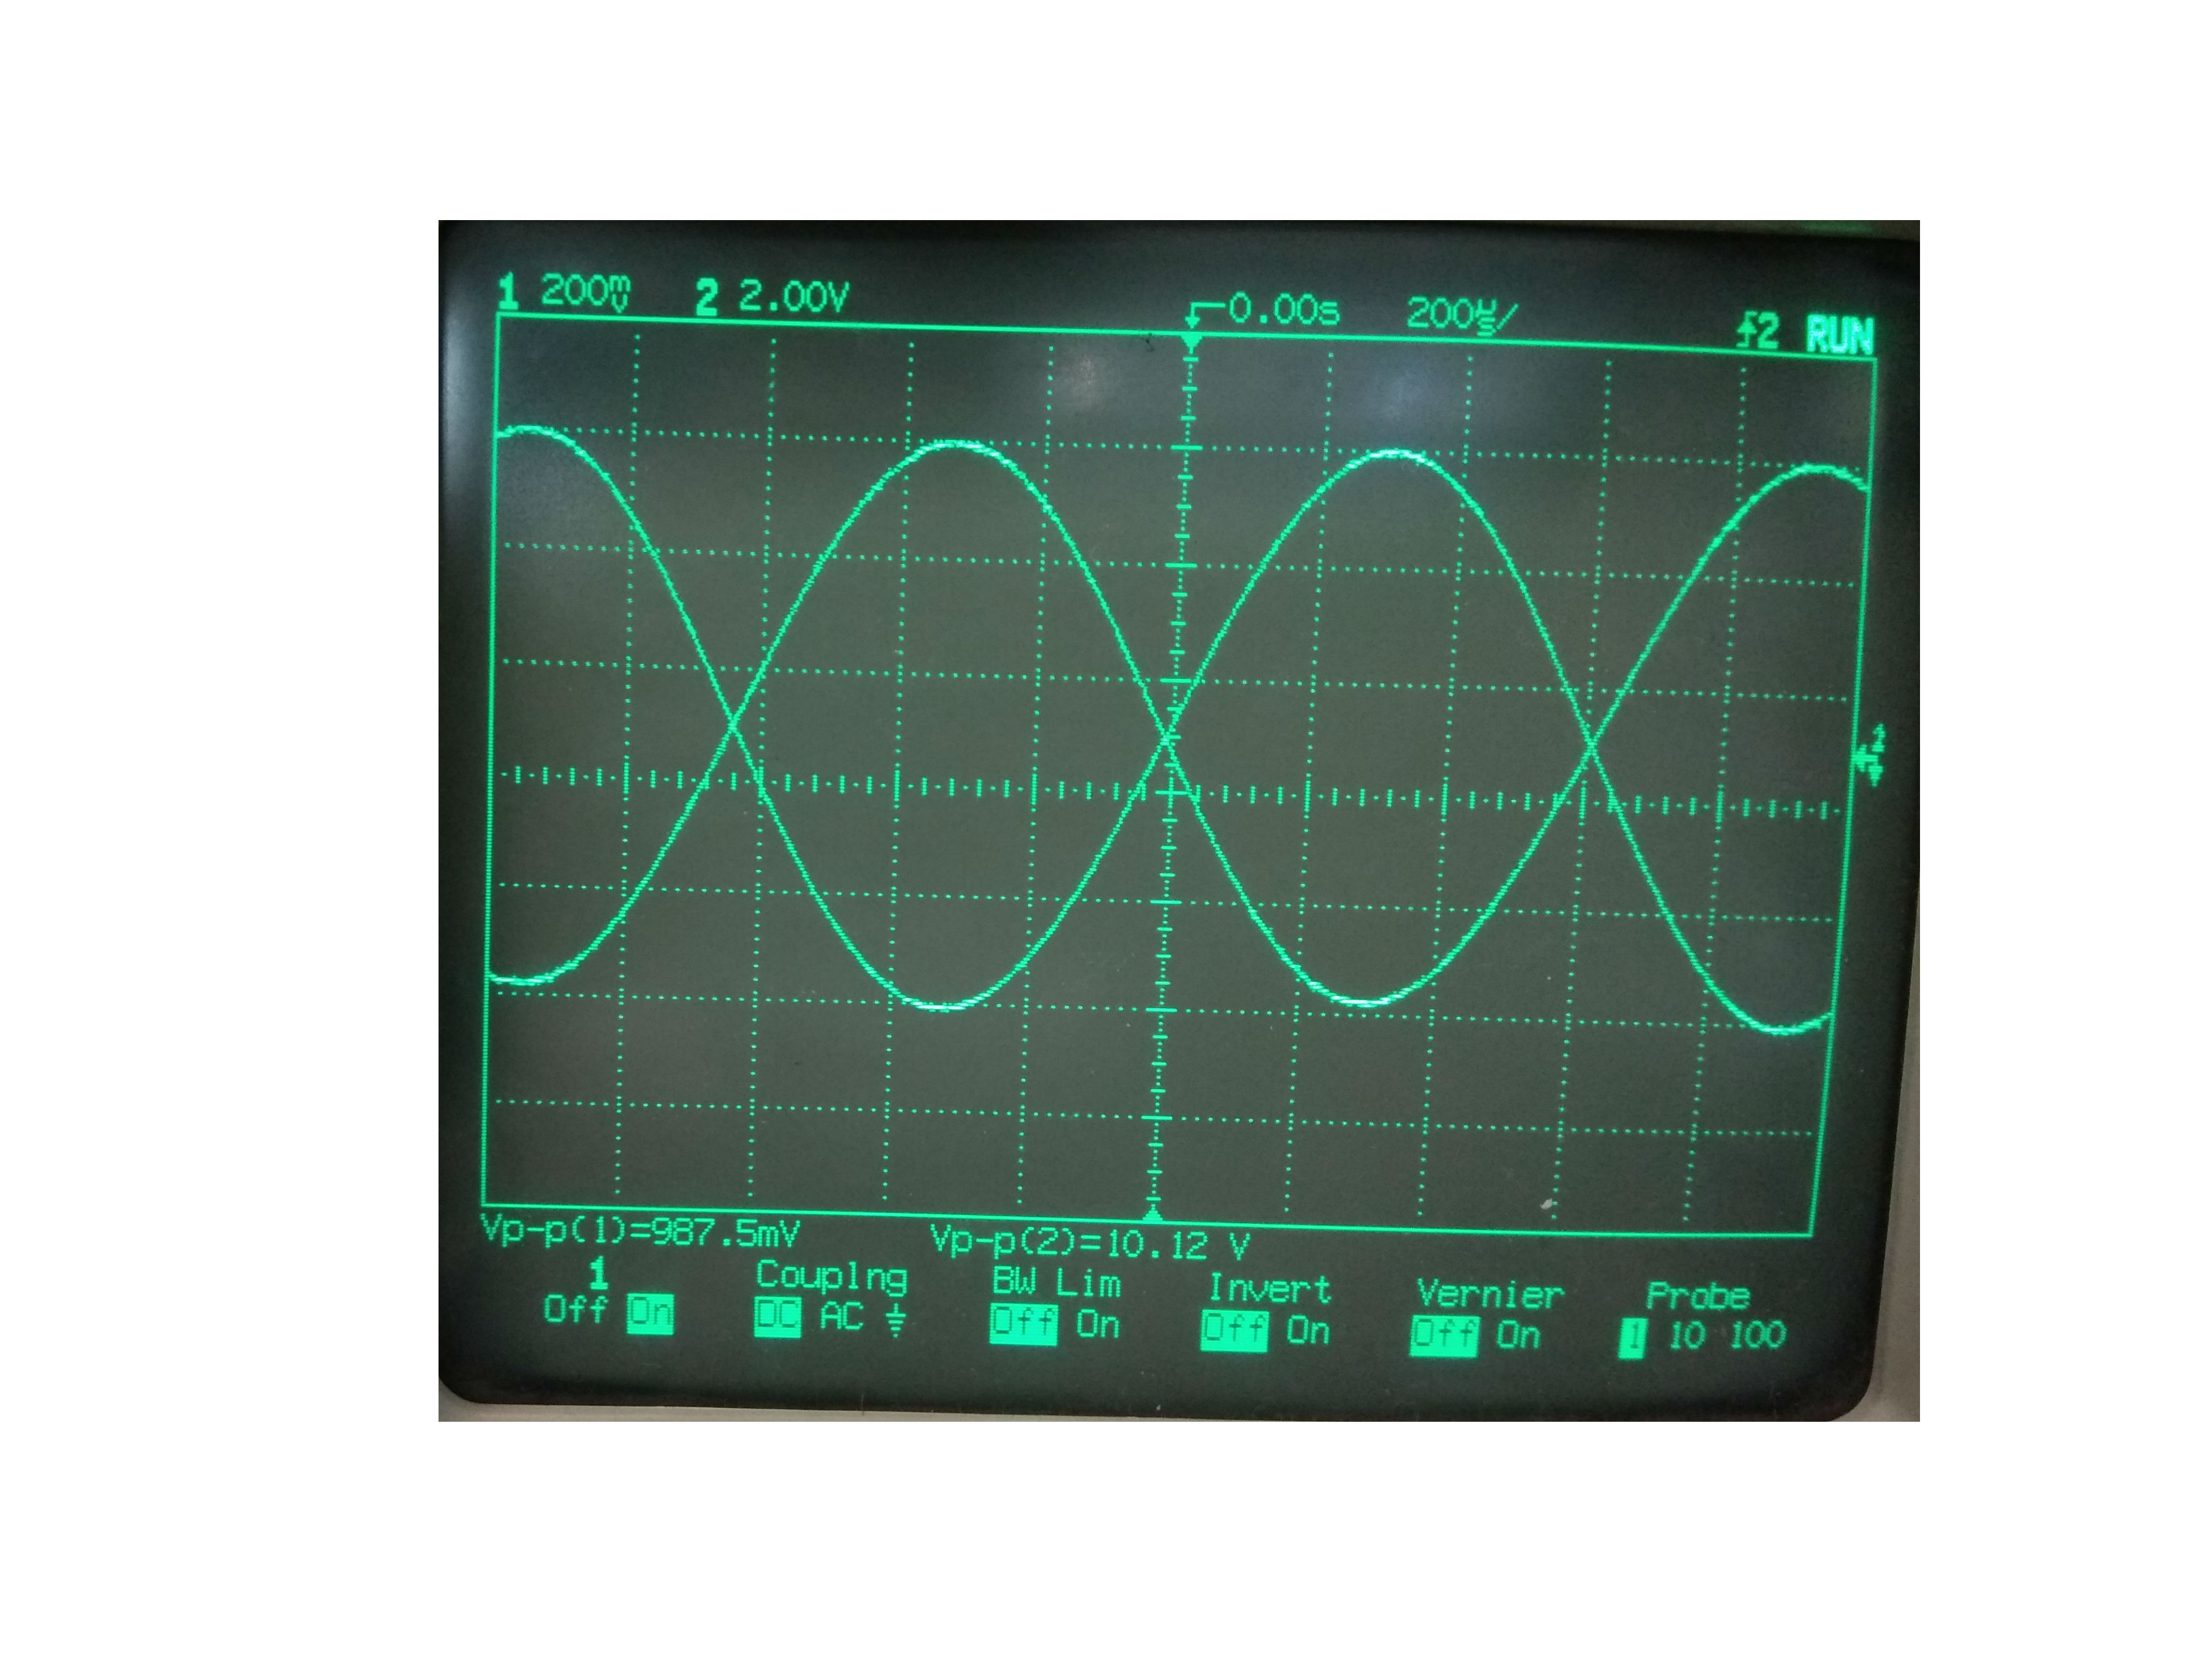
\includegraphics[width=\textwidth]{fase.jpg}
  \caption{Inversione di fase}
  \label{fig:invfase1}
\end{figure}

\end{document}
